\documentclass[oneside,12pt]{Classes/VTU}
\usepackage{fancyhdr}
\usepackage{multicol}
\usepackage{geometry}
\usepackage{wrapfig}
\usepackage{graphicx}
\usepackage{tabularx}

\makeatletter
\def\headrule{{%
		\if@fancyplain\let\headrulewidth\plainheadrulewidth\fi
		\hrule\@height\footrulewidth\@width\headwidth\vskip1pt%
		\hrule\@height\headrulewidth\@width\headwidth\vskip-\headrulewidth\vskip-4pt
}}
%
\def\footrule{{%
		\if@fancyplain\let\footrulewidth\plainfootrulewidth\fi
		\vskip-\footruleskip\vskip-\footrulewidth
		\hrule\@height\headrulewidth\@width\headwidth\vskip1pt%
		\hrule\@height\footrulewidth\@width\headwidth\vskip\footruleskip
}}

\renewcommand{\headrulewidth}{0.4pt}
\renewcommand{\footrulewidth}{0.4pt}

\hbadness=10000
\hfuzz=50pt

%\usepackage{StyleFiles/watermark}
\usepackage{multirow}
\usepackage{epsfig}
\usepackage{enumerate}
\usepackage{amsmath}
\usepackage{amsthm}
\usepackage{amscd}
\usepackage{amssymb}
\usepackage{rotating}
\usepackage{graphicx}
\usepackage{algorithm}
\usepackage{algorithmic}
\usepackage{setspace}
\usepackage[T1]{fontenc}
\usepackage{alltt}
\usepackage{array}
\usepackage{pdfpages}
\usepackage{makecell}


\begin{document}
	\pagenumbering{roman}
	\lhead{An Online Scalable Low Latency Multiplayer Game Using Docker}
	\rhead{AY: 2021-2022}
	\lfoot{Department of Computer Science and Engineering}
	\rfoot{\thepage}
	\cfoot{}
	
	\renewcommand\baselinestretch{1.2}
	\baselineskip=18pt plus1pt
	
	%\maketitle
	
	\setcounter{secnumdepth}{3}
	\setcounter{tocdepth}{3}
	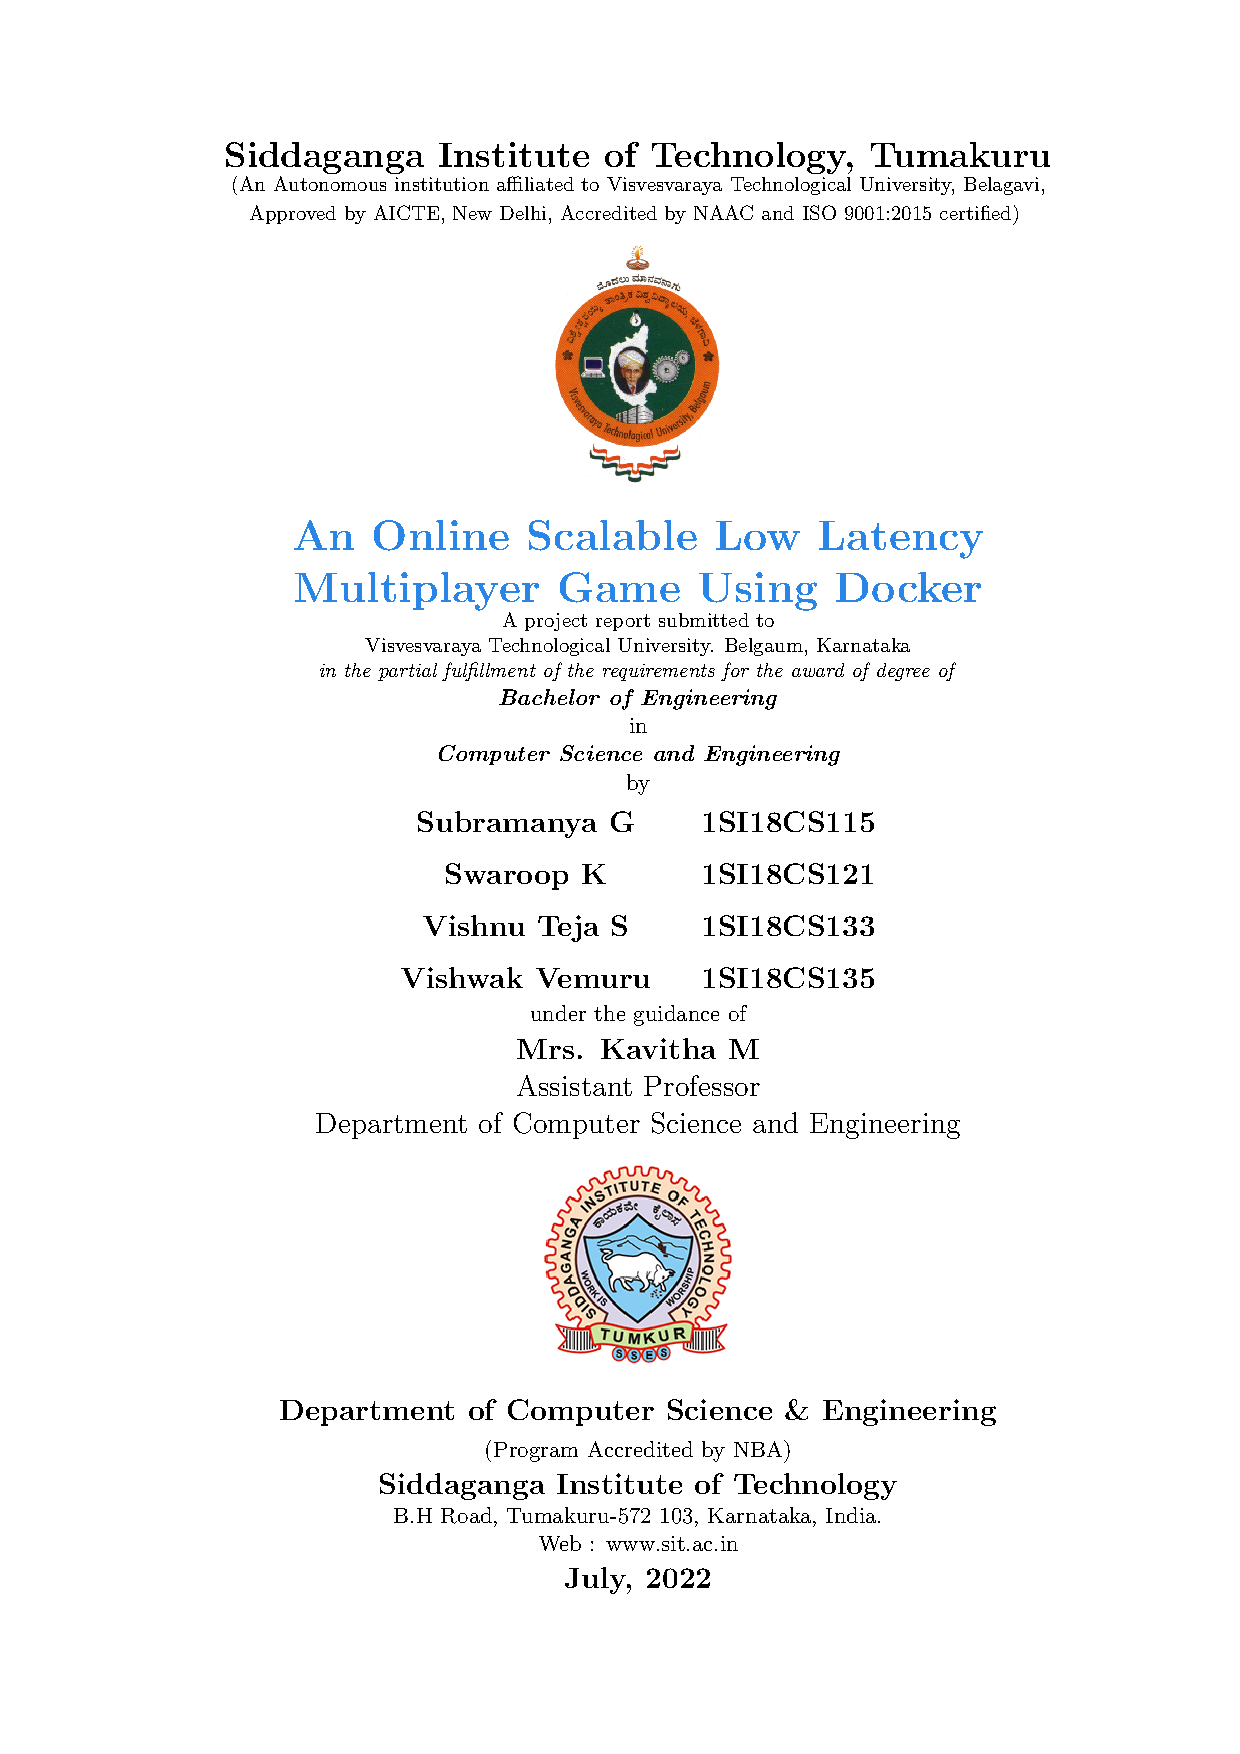
\includepdf[pages=-]{FrontPage.pdf}
	
	\begin{center}
		\bfseries
		\large{Department of Computer Science and Engineering\\
			Siddaganga Institute of Technology, Tumakuru - 572103} \\
		\begin{figure}[hbtp]
			\centering
			
\includegraphics[scale=1]{sit.png}
		\end{figure}
		\LARGE{DECLARATION} \\
	\end{center}
	\vspace{0.5in}
	\normalsize{
		We hereby declare that the entire work embodied in this dissertation has been carried out by us at \textbf{Siddaganga Institute of Technology} under the supervision of \textbf{Mrs. Kavitha M}, Asst. Professor, Department of Computer Science and Engineering. This dissertation has not been submitted in part or full for the award of any diploma or degree of this or any other University.} \\
	\vspace{0.5in}
	\begin{flushleft}
		\begin{enumerate}
			\item Subramanya G (1SI18CS115)
			\item Swaroop K (1SI18CS121)
			\item Vishnu Teja S (1SI18CS133)
			\item Vishwak Vemuru (1SI18CS135)
		\end{enumerate}
	\end{flushleft}
	
	\pagebreak
	\begin{center}
		\textbf{\LARGE{Acknowledgements}}
	\end{center}
	\addcontentsline{toc}{chapter}{Acknowledgements}
	\begin{enumerate}[]
		\item With reverential pranams, we express our sincere gratitude and salutations to his holiness, \textbf{Dr. Sree Sree Shivakumara Swamigalu}, Founder President, \textbf{Sree Sree Siddalinga Swamigalu}, President, Sree Siddaganga Math, for being a constant source of inspiration in the course of study.
		\item First and foremost, we wish to express our deep sincere feeling of gratitude to our institution, \textbf{Siddaganga Institute of Technology}, for providing us an opportunity for completing our project successfully.
		\item We are grateful to \textbf{Dr. M N Channabasappa}, Director, Siddaganga Institute of Technology, Tumakuru for his kind cooperation and encouragement.
		\item We express our kind thanks to \textbf{Dr. S.V. Dinesh}, Principal, Siddaganga Institute of Technology, Tumakuru for his encouragement.
		\item We express our heartfelt thanks to \textbf{Dr. A S Poornima}, Professor and Head, Department of Computer Science and Engineering, Siddaganga Institute of Technology, Tumakuru for her valuable suggestions and advice.
		\item We express our heart full gratitude and humble thanks to our project guide \textbf{Mrs. Kavitha M}, Asst. Professor, Department of Computer Science and Engineering, Tumakuru for guiding and facilitating us to complete the major project work successfully.
		\item We would also like to thank all the panel members of the project for their scrutiny throughout the various stages of evaluations and presentations. Without their appropriate questioning and guidance, the project would not have been completed.
		\item We are conscious of the fact that, we have received cooperation in many ways from the Teaching, Technical and supporting staffs of the Department of Computer Science and Engineering and we are grateful to all for their cooperation. We would also like to thank our friends and family for being a constant source of moral support and encouragement throughout the project.
	\end{enumerate}
	
	\tableofcontents
	\pagebreak
	\addcontentsline{toc}{chapter}{Abstract}
	\thispagestyle{fancy}
	
	\section*{Abstract}
		\thispagestyle{fancy}
		
		\paragraph{\normalfont{An online multiplayer game allows users from across the world to connect and play together. Most modern multiplayer games use the client-server architecture. However, in these types of online games, there are issues of latency and performance. To solve these issues, we are building an online scalable low latency multiplayer game using Docker containers. Docker containers can be deployed on a cloud nearest to the client reducing latency and they also enable easy management of game servers. }}
		
		\paragraph{\normalfont{The game would be implemented in the form of a web application. The basic architecture consists of the game as a client-server model. Any number of clients can join the server and each client has their own game instance in the server, grouped under rooms. A cluster of docker containers are used to run the server. We make use of the Phaser game framework to render the game, maintain the game state and we use MongoDB for the database. The Docker containers will be hosted on a cloud. }}
		
		\paragraph{\normalfont{The game will be able to provide cross-platform support. The game would be a fast-paced combat game and will be able to establish real time communication between the user game-play session and the server. The game will also be able to allow users to create private and public rooms for game sessions and the game server will run on docker containers. }}
		
	\thispagestyle{fancy}
	\listoffigures
	\thispagestyle{fancy}
	\addcontentsline{toc}{chapter}{\listfigurename}
	\newpage
	\pagenumbering{arabic}
	
	\chapter{Introduction}
	\thispagestyle{fancy}
		\section{Background Study}
			\thispagestyle{fancy}
			\paragraph{\normalfont{A multiplayer game is one in which more than one person can play in the same game environment at the same time, either locally and on the same computing system, locally and on different computing systems via a local area network, or locally and on different computing systems via a wide area network, most commonly the Internet.}}
			
			\paragraph{\normalfont{The game will be having the following features:}}
			\begin{itemize}
				\item Orthogonal Top-down view
				\item Co-op Combat
				\item Character Customization
				\item Public and private rooms for game sessions
			\end{itemize}
			\paragraph{\normalfont{The types of multiplayer games are: }}
			\begin{enumerate}
				\item Non-networked Games: These are predominantly 2-player games played on a single device with multiple controllers.
				\item Networked Games: These allow users from different devices to connect to each other and play the games. It has following two categories: 
				\begin{enumerate}[a.]
					\item Local Multiplayer: They are always played on the same local network.
					\item Online Multiplayer: They Can be played through any device across the Internet.
				\end{enumerate}
			\end{enumerate}
			
			\paragraph{\normalfont{The game would be an online multiplayer game where players are not restricted to the same network. This can be implemented in two ways as follows:}}
			\begin{enumerate}
				\item Peer-to-Peer: In these types of games, one of the players become the authority and all other players has to send the data to the authoritative person. The authority updates the game states and sends the updated states to all the other players. Peer-to-Peer type of game has the following disadvantages:
				\begin{itemize}
					\item The peer who becomes the authority has to have a large bandwidth.
					\item If the authoritative peer exits, the game automatically ends for all players. 
					\item Peer server can change the states, which affects the playing experience for all players.
				\end{itemize}
				\item Client Server: In these types of games, a dedicated server is set up. All clients must connect to this server and the server is the authority. This successfully overcomes all the disadvantages of the Peer-to-Peer types of online multiplayer games. 
			\end{enumerate}
			
			\paragraph{\normalfont{Most modern multiplayer games use the client-server architecture. However, in these types of online games, there are issues of latency and performance.  The primary causes of latency are and other performance issues are:}}
			\begin{itemize}
				\item Bandwidth: Online multiplayer games generally requires a high bandwidth.
				\item Wired connections have low latency than Wireless connections. 
				\item Internet network hardware.
				\item Remote server locations and connections used by remote server.
				\item Internet service provider. 
				\item Network Interference. 
			\end{itemize}
			
			\paragraph{\normalfont{The solution to the above problems is to use docker containers. Docker is an open platform for app development, shipping, and running. Docker allows us to decouple our apps from our infrastructure, allowing us to release software swiftly.  Docker allows us to bundle and run an application in a container, which is a loosely isolated environment. Because of the isolation and security, we can run multiple containers on a single host at the same time. Containers are lightweight and include everything required to run a program, eliminating the need to rely on what is currently installed on the host. }}
			
			\paragraph{\normalfont{Docker provides a container life-cycle management platform and related tooling and thus:}}
			\begin{itemize}
				\item Containers are used to develop applications and their supporting components. 
				\item The container serves as the distribution and testing unit for applications. 
				\item Allows deploying of applications as containers or orchestrated services into a production environment. It provides the same experience  irrespective of the production environment being a local data centre, or a cloud provider, or a hybrid of the two.
			\end{itemize}
			
			\paragraph{\normalfont{In the case of online multiplayer game, docker enables easy management of game servers and allows for deployment on the cloud. This allows an instance of the game to run on the nearest cloud server to the user solving the issues of latency. As there are multiple docker containers running the server, the performance is boosted. Further, using docker containers enables support for rolling deployment, auto-scaling, monitoring and maintenance of the game server.}}
			
		\section{Related Works}
		
			\subsection{Pokémon GO}
				%plagia tegibeku
				\paragraph{\normalfont{Pokémon Go is an augmented reality (AR) mobile game released in 2016 as part of the Pokémon series by Niantic in conjunction with Nintendo and The Pokémon Company for iOS and Android devices. It use GPS-enabled mobile devices to identify, capture, train, and battle virtual monsters known as Pokémon, who appear to be in the player's real-world location. The game began with approximately 150 Pokémon species, which had grown to approximately 700 by 2021. Pokémon Go uses many services across google cloud, cloud data-store acting as game's primary database for storing the game world.}}
								
				\begin{figure}[t]
					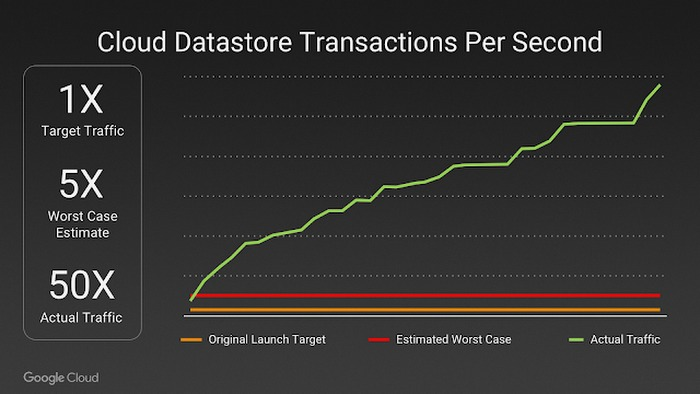
\includegraphics[scale=0.5]{pokemonGO.jpeg}
					\centering
					\caption{Graph depicting a surge in the number of transactions of Pokémon Go}
					\label{fig:poke}
				\end{figure}
				
				\paragraph{\normalfont{The graph in Fig. \ref{fig:poke} portrays the transactions per second estimated and witnessed by the Niantic team. They targeted 1X player traffic, with a worst-case estimate of nearly 5X that target. Pokémon GO’s popularity quickly surged player traffic to 50X the initial target, ten times the worst-case estimate. In response the Google CRE (Customer Reliability Engineering) team had to provision extra capacity on behalf of Niantic to keep up with this surge.}}
				
				\paragraph{\normalfont{Pokémon GO, in addition to being a global craze, is one of the most fascinating examples of container-based development in the wild. The game's application logic runs on Google Kubernetes Engine (GKE), which is powered by the open source Kubernetes project. Niantic picked GKE so that their team could concentrate on releasing live modifications to its players. Niantic leveraged Google Cloud in this way to transform Pokémon GO into a service for millions of players, constantly changing and improving.}}
				
			\subsection{Super Mario}
				\paragraph{\normalfont{Super Mario is a 2D and 3D platform game series created by Nintendo based on and starring the fictional plumber Mario. At least one Super Mario game has been released for every major Nintendo video game console. There are over twenty games in the series}}
				
				\paragraph{\normalfont{\emph{PengBAI}, a docker hub user, has made a fan game of Super Mario called Infinite Mario using HTML5 JavaScript. They have made use of docker to distribute this fan game and allow others to play the game. This work is similar to our project but it only makes use of docker as a distribution mechanism and does not aim to perform any optimisations for having better latencies. This game only has a support for a single player and completely runs on the client side. }}
				
			\subsection{Minecraft}
				\paragraph{\normalfont{Minecraft is a 3D sandbox game originally created by Markus "Notch" Persson. It is maintained by Mojang Studios, a part of Xbox Game Studios, which in turn is part of Microsoft. One of the simplest examples that people have used over the years of demoing Docker is quickly standing up and running a Minecraft server. This shows the power of using Docker and has a pretty practical application.}}
				
				\paragraph{\normalfont{There are various images in docker hub for Minecraft servers with various configurations, however, each instance of the server runs on only one container making scalability an issue. }}
				
			\subsection{Among Us}
				\paragraph{\normalfont{Among Us is a 2018 online multiplayer social deduction game developed and published by American game studio Innersloth. The game was inspired by the party game Mafia and the science fiction horror film The Thing. The game allows for cross-platform play, first being released on iOS and Android devices. }}
				
				\paragraph{\normalfont{Among Us is a classic example of an online multiplayer game. It provides support for public and private rooms, i.e., players can play the game together with a group of friends in the private instance of the game or connect to public instances to play with strangers. The game server is hosted in North America, Asia and Europe to provide more connectivity, however, the game is not containerized and thus can not run on nearest cloud server available to the player. }}
		
		\section{Problem Statement and objectives}
			\thispagestyle{fancy}
			\textbf{Problem Statement: }
			To develop an Online Scalable Low Latency Multiplayer Game Using Docker
			\newline
			\newline
			\newline
			\textbf{Objectives:}
			\newline
			\begin{itemize}
				\item To enable cross-platform support by building a web application.
				\item To build a fast-paced combat game.
				\item To establish a two-way interactive communication session between a user's browser and a server in real time.
				\item To enable users to create private and public rooms for game sessions.
				\item To containerize the game server and reduce the game server overhead.
				
			\end{itemize}
		
		\section{Organization of the Report}
			This report is organized into six chapters followed by a Bibliography section as follows: 
			
			\paragraph{\normalfont{Chapter 1 provides an overview of the project. It covers relevant works that are similar to ours and served as inspirations for creating this project. This chapter also contains the problem statement and the work objectives.}}
			
			\paragraph{\normalfont{Chapter 2 contains a literature review, in which we detail all of the technical articles that we have read in order to better grasp the concepts behind this project and come up with relevant changes and features to add.}}
			
			\paragraph{\normalfont{Chapter 3 interprets the system's high-level design. This section also includes the project's architecture, functional requirements, non-functional requirements, and software development process used.}}
			
			\paragraph{\normalfont{Chapter 4 focuses on the project's implementation phase. It discusses the tools and technologies used in the project, as well as the project's implementation procedure.}}
			
			\paragraph{\normalfont{The details of the test scenarios we evaluated for testing our application are presented in Chapter 5. It also includes a results section where the work's output is documented.}}
			
			\paragraph{\normalfont{The conclusion to the project is presented in Chapter 6. It also includes potential future work connected to this project.}}
	
	\chapter{Literature Survey}
		\thispagestyle{fancy}
		
		\paragraph{\normalfont{Many works and papers were referred and the following things were noted.}}
		
		
		\paragraph{\normalfont{Cloud gaming is the gaming industry's future, allowing consumers to play games from any location, at any time, and on any device. The research \cite{paper1} covers the two key difficulties in cloud gaming: resource allocation and maintaining user experience quality. \cite{paper1} also discusses how to improve cloud gaming performance by initialising the cloud gaming package inside Docker containers, which will allow the application to be more reliable by secularising its resource allocation and increasing the overall performance of the cloud gaming system while utilising fewer resources.}}
		
		\paragraph{\normalfont{The real-time strategy game StartCraft: Brood War is a popular area for AI study, with a pre-installed library of AI programming tools supporting all major StarCraft bot kinds. \cite{paper2} shows a Dockered version of StarCraft.Despite StarCraft's restricted OS support, the implementation in \cite{paper2} provides an easy way to deploy StarCraft AIs on several hosts at once and across multiple platforms. \cite{paper2} also covers the Docker image design and shows a few use scenarios.}}
		
		\paragraph{\normalfont{Mobile Edge Computing (MEC) is a new network paradigm that provides cloud and IT services at the network's point of access. Such proximity to the end user results in ultra-low latency and high bandwidth, while also reducing the congestion in the network core. Because servers must be run on edge nodes, a major component of MEC systems is server mobility and low overhead. \cite{paper3} suggests using Docker as a tool for this purpose. Docker is a technology that enables the quick and easy deployment of Linux containers. \cite{paper3} investigates Docker's usefulness in MEC settings by quantifying the CPU utilised by Docker when operating two different containerized services: multiplayer gaming and video streaming. The authors' tests with varying numbers of clients and servers in \cite{paper3} yield different results for the two case studies: for the gaming service, the overhead logged by Docker increases only with the number of servers; for the video streaming case, the overhead is unaffected by the number of either clients or servers.}}
		
		\paragraph{\normalfont{Recent advancements in cloud computing enable cloud gaming to give users with a high-end quality of experience. \cite{paper4} asserts that the fundamental requirement of gaming is to deliver the best possible gamer experience; nevertheless, cloud gaming falls short in this regard because the network transmission of game scenes from cloud game server to gamer device is long. Through this study, the author hopes to reduce latency and improve performance in cloud gaming. Based on the Node selection algorithm, \cite{paper4} recommends shifting the cloud game server to the fog nodes located at the player's edge network. \cite{paper4} also advises that traditional virtual machines be replaced by lightweight containers to improve cloud gaming performance.}}
		
		\paragraph{\normalfont{HTML5 has given many developers the opportunity to explore with new web development options. The authors' goal with \cite{paper5} is to provide a high-level summary of what this entails for the game development community. \cite{paper5} assesses new HTML5 and JavaScript elements. It also emphasises WebGL, Canvas, and WebSockets, which have enabled developers to expand their creativity by modifying images, generating 3D worlds, and allowing real-time interactivity.}}
		
		\paragraph{\normalfont{Big Two is a multiplayer online game featuring erroneous facts. Each player in this game plays without knowing the opponent's confidential information. \cite{paper6} uses Big Two as an example to demonstrate the requirement for web-based multiplayer games with imperfect information to have real-time communication in order to handle rapid information changes and the game state at any time. \cite{paper6} suggests a new architecture for web-based multiplayer games with incomplete information. \cite{paper6} uses an open-source WebSocket, Socket.IO, as a case study and implements this framework in Big Two.}}
	
	\chapter{High-level Design}
	\thispagestyle{fancy}
		\section{Software development Methodology}
			\subsection{Agile Methodology}
				\begin{figure}[H]
					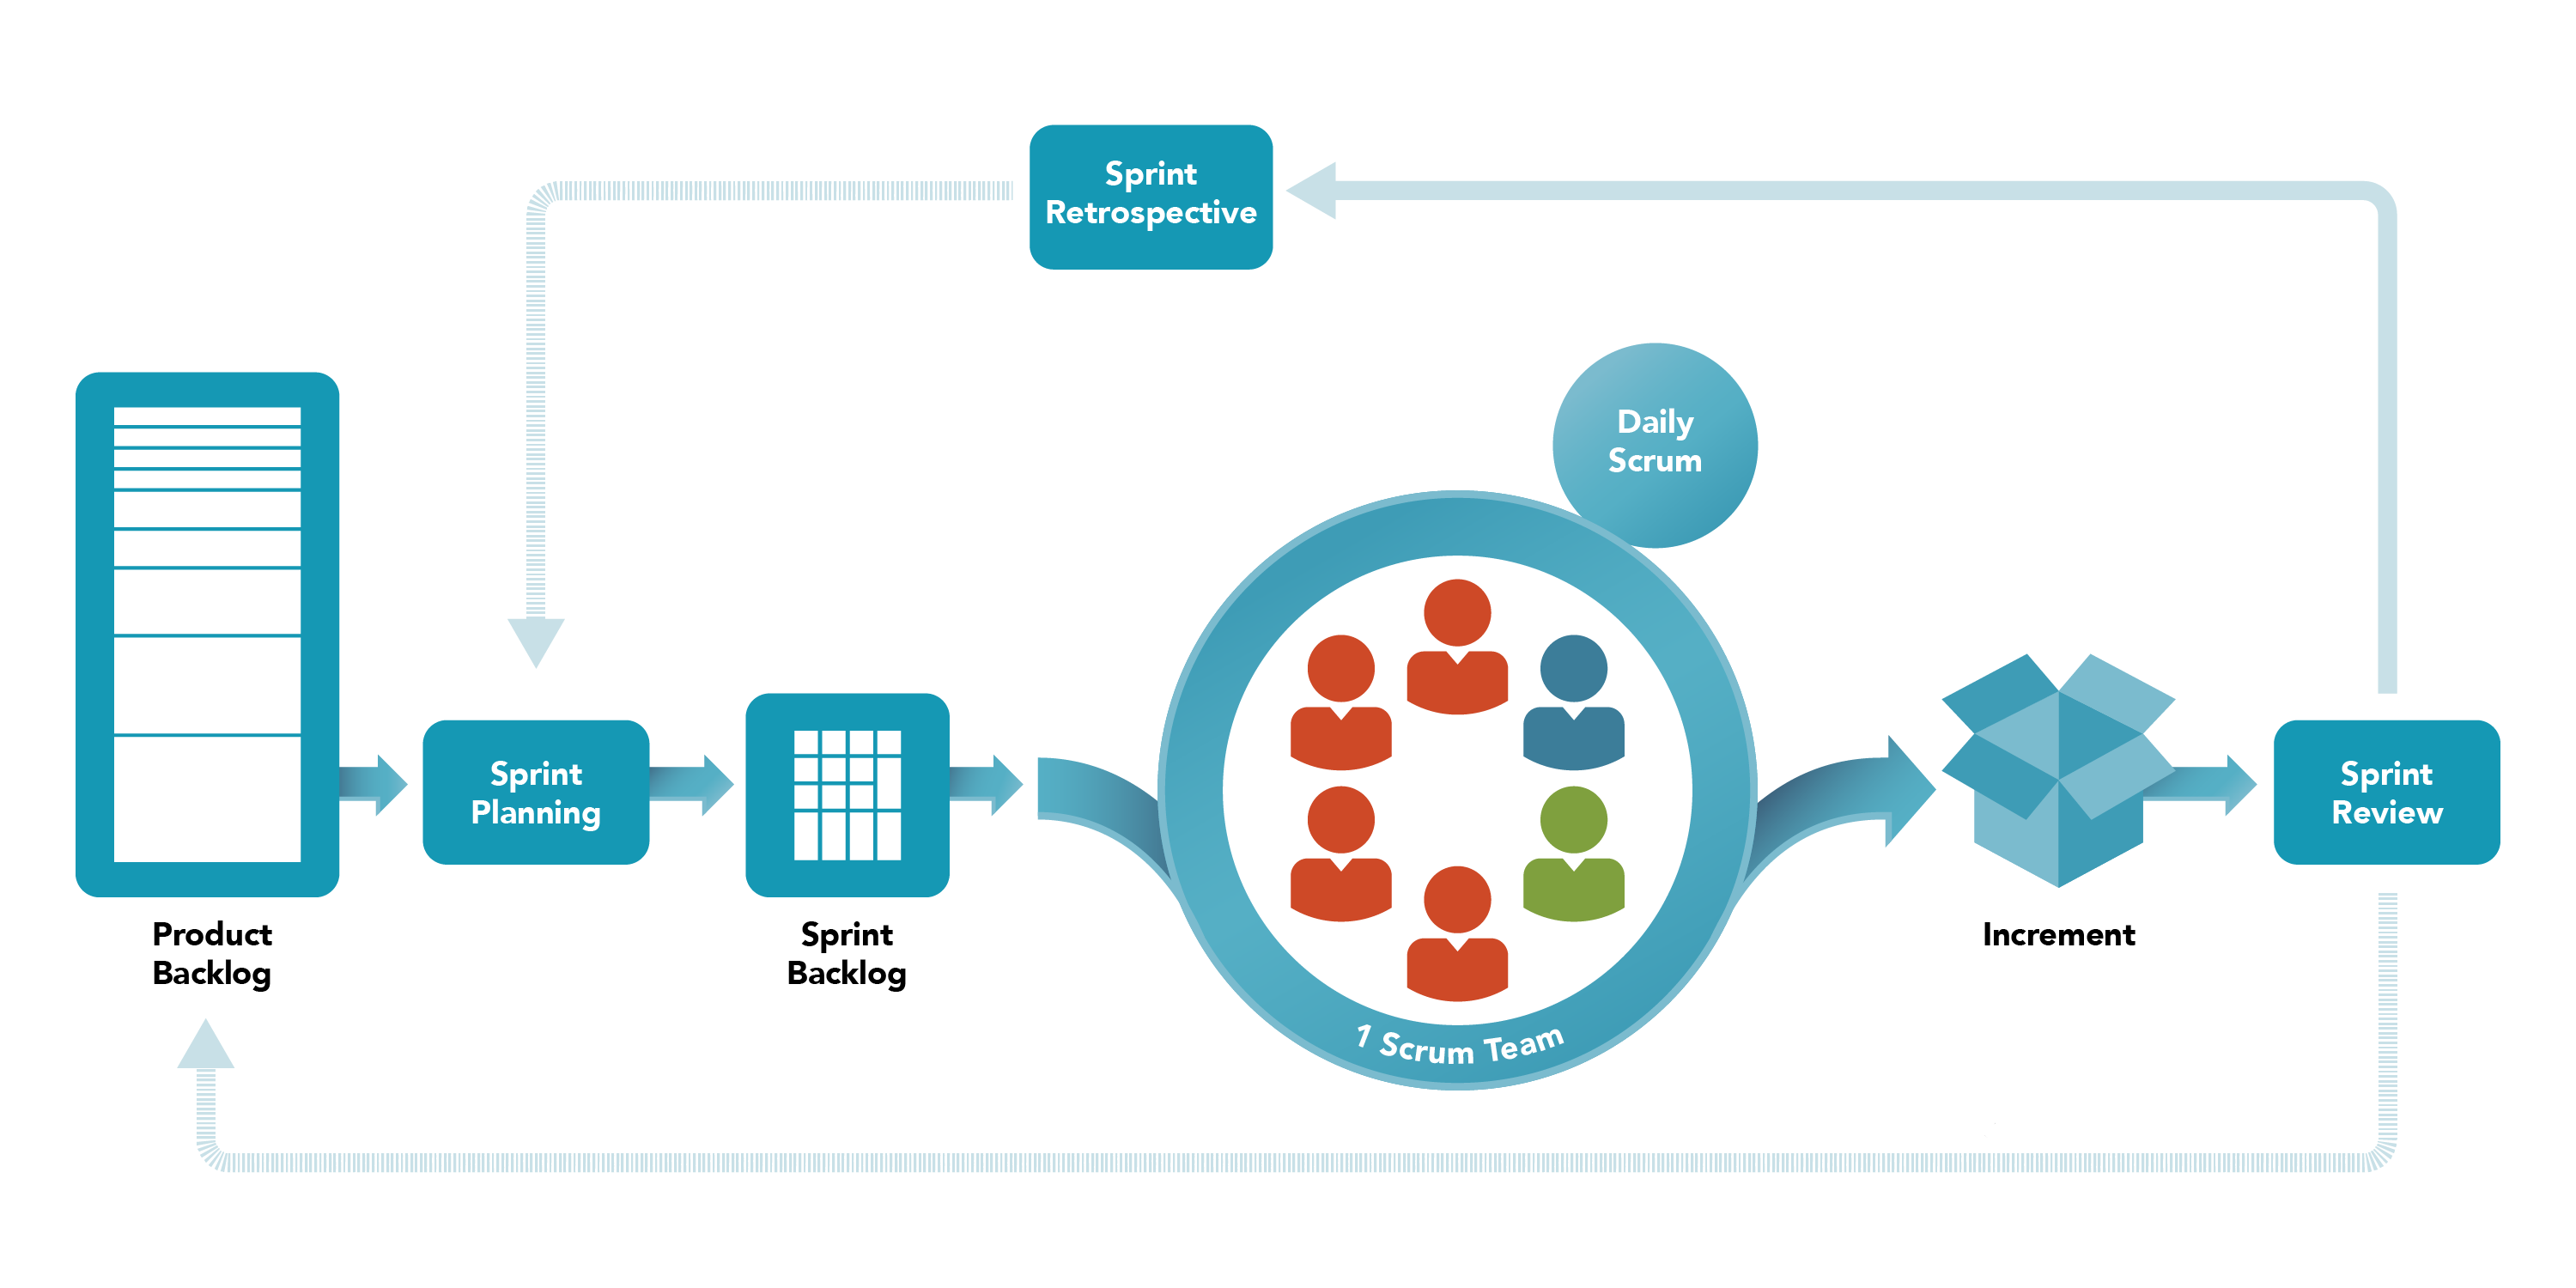
\includegraphics[width=15cm]{agile1.png}
					\centering
					\caption{Figure showing the Agile software development methodology}
					\label{fig:a1}
				\end{figure}
				
				\begin{figure}[H]
					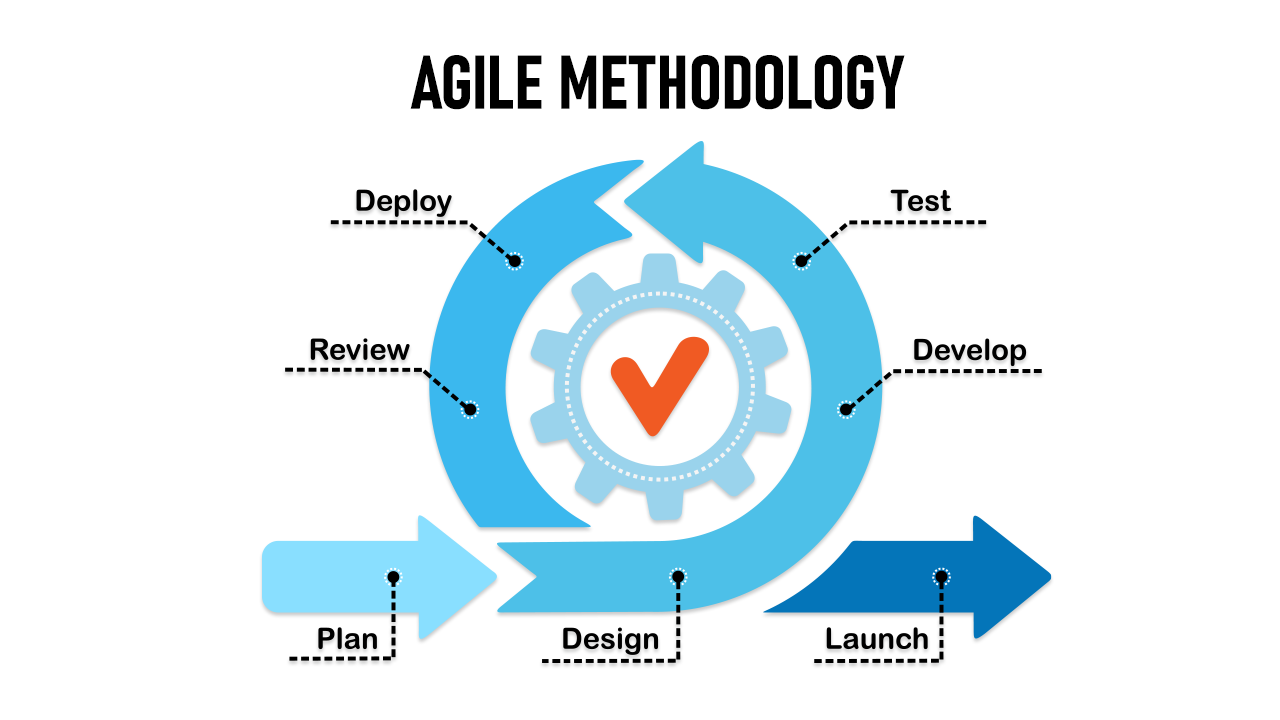
\includegraphics[width=15cm]{agile2.png}
					\centering
					\caption{Figure showing the steps involved in the Agile model}
					\label{fig:a2}
				\end{figure}
				
				\paragraph{\normalfont{The Agile methodology is a  project management technique that focuses on building a project iteratively by dividing it into small deliverable stages. At each stage, it requires continuous collaboration and progress. When the job begins, agile teams go through the cycle of planning, execution, and evaluation. }}
				
				\paragraph{\normalfont{Fig. \ref{fig:a1} shows the agile methodology. The product backlog is prepared after requirement analysis and is consists of all the features that are to be implemented in the project. A sprint is a brief period of time during which a team works to complete a specific amount of work. A sprint backlog is then prepared from the product backlog which consists of the tasks to be completed in a particular sprint. This process is referred to as sprint planning. }}
				
				\paragraph{\normalfont{The following activities happen within a sprint cycle as shown in Fig. \ref{fig:a2}: }}
				\begin{itemize}
					\item Plan
					\item Design
					\item Develop
					\item Test
					\item Deploy
					\item Review
					\item Launch
				\end{itemize}
			
				\paragraph{\normalfont{The sprint cycles are repeated for each increment of the project. }}
			
			\subsection{Why Agile for our project?}
				\paragraph{\normalfont{We have made use of the Agile methodology for the development of this project as it offers the following advantages over traditional methods: }}	
				
				\begin{itemize}
					\item Agile enables teams to deliver a prototype and iteratively enhance it with each cycle.
					
					\item Agile enables teams and individuals to prioritise features more effectively.
					
					\item Agile techniques encourages reactive decisions, shorten development periods, and enable just-in-time request analysis.
					
					\item Based on the test results, teams can make immediate course adjustments.
				\end{itemize}
		
		\section{Architecture}
			
			\begin{figure}[H]
				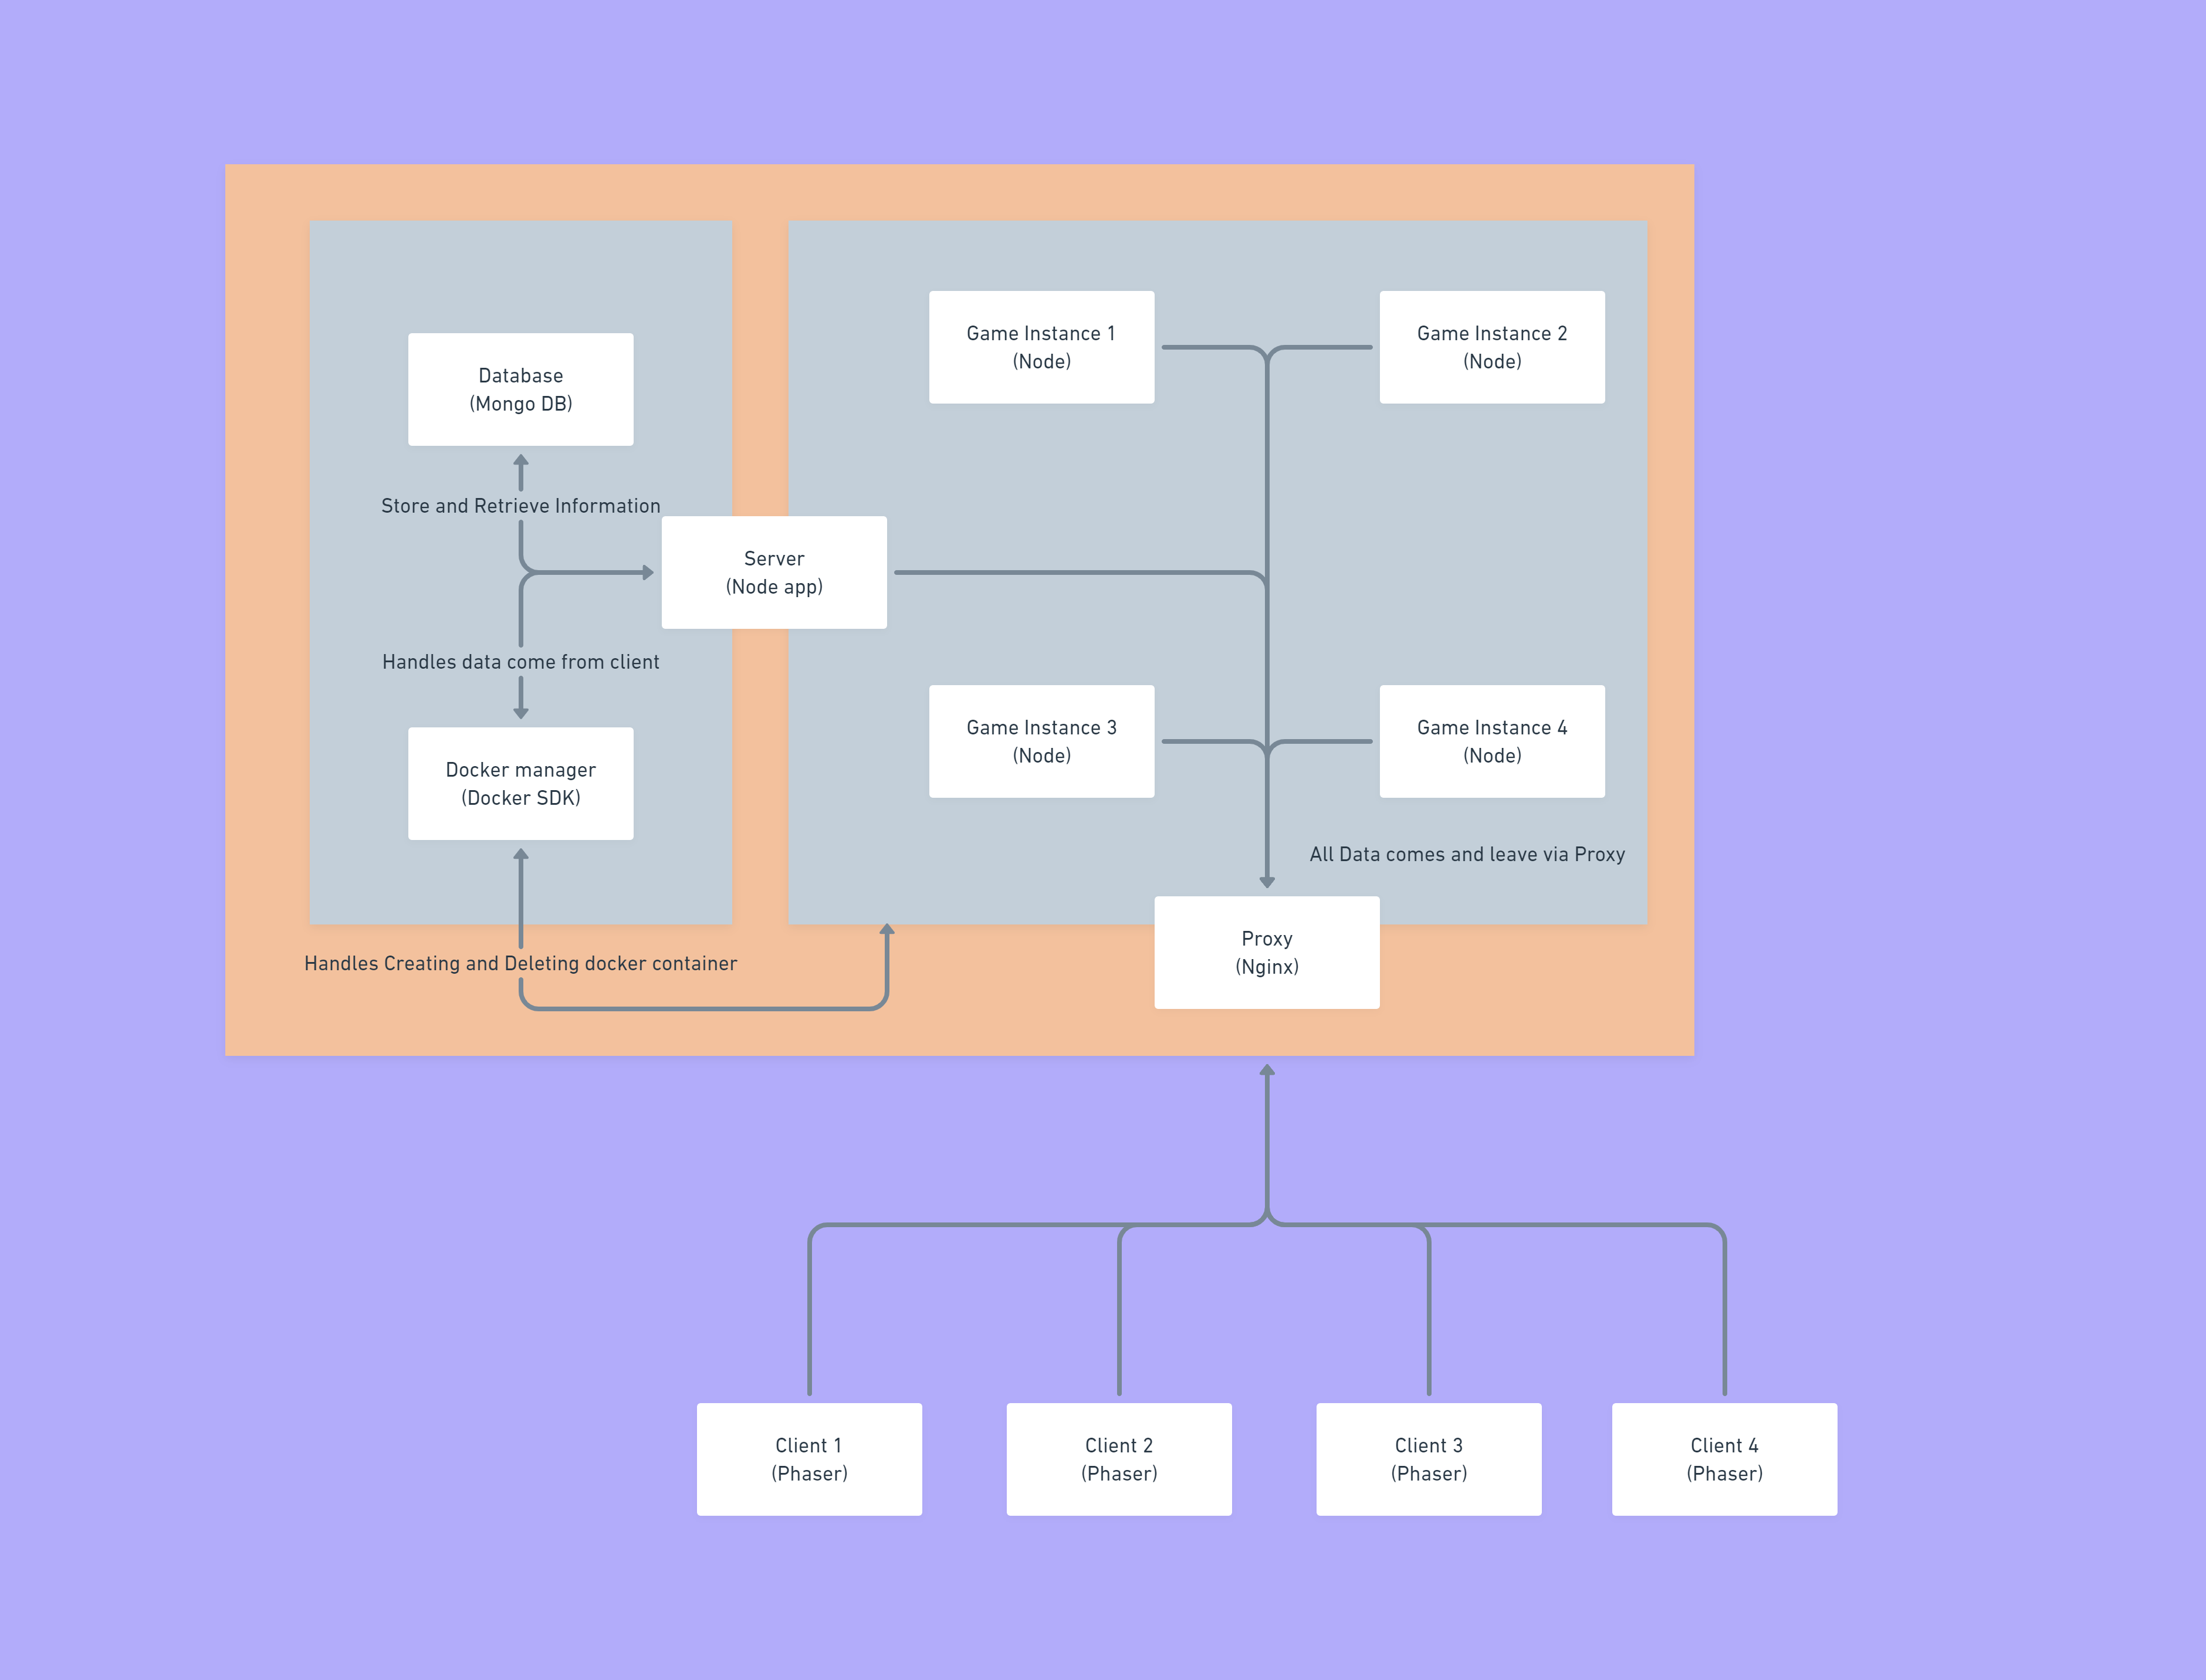
\includegraphics[width=12cm]{archi.png}
				\centering
				\caption{Figure showing the architecture for the project}
				\label{fig:archi}
			\end{figure}
		
			\paragraph{\normalfont{The architecture of a system describes its structure and behaviour. It also comprises a graphical depiction of the ideas, concepts, elements, and components of the system.}}	
		
			\paragraph{\normalfont{The following are the major components of the architecture of our project as shown in Fig. \ref{fig:archi}: }}
			\begin{enumerate}
				\item \textbf{Database:} In this project we make use of MongoDB database. MongoDB is a cross-platform database, classified as a NoSQL database. It uses JSON like documents with optional schema. We use this database primarily to store the state of the game. We store the state for each room (A room represents a group of users playing together) which a group of users connect to. We store the room ID, the members of the room, their characters and respective inventory ie., the weapons, coins collected etc. 
				
				\item \textbf{Docker Manager:} Docker is a set of platform-as-a-service products that use OS-level virtualization to deliver software in packages called containers. Docker manager is a tool that runs the docker SDK. It helps us to create and manage the various rooms in the game. Each docker instance will run a single instance of the game. The database and the docker manager constitute the backend of our application. 
				
				\item \textbf{Server:} The server uses Node.js to connect to the docker containers running the game to the users. Node.js is an open-source, cross-platform backend JavaScript runtime environment that runs on the V8 engine and executes the JavaScript code outside the web browser. It acts as a middleware between backend and frontend. It provides a layer of abstraction between the database and docker manager. It also manages the user authentication. 
				
				\item \textbf{Game Instance:} It is a docker container that is created and managed by the docker manager. It acts as the frontend. Each game instance runs a game server within a docker container which the players can join. It manages the users who have joined, broadcasts the game state to all the users and creates the maps of the game procedurally. 
				
				\item \textbf{Proxy(Nginx)}: Each user connecting to the application must connect to the containers through different ports. But, the number of ports available ports is limited - there are 65535 ports out of which 2000 are meant for special purposes. As a result of which we need something that maps each container to the outside world. The advantage of using docker is that, a user can connect to a docker instance or container using its name. So we use a proxy that maps the external request of the user to the internal network. In our application, the proxy works by mapping a request with subdomain having the name of a docker instance to that particular docker instance. For example, \emph{domain.com/abc} connects to the \emph{abc} container. 
				
				\item \textbf{Client:} The client program uses the Phaser game engine and it runs on the browser of the user. The specifics of the game are written in TypeScript files. The client obtains the data from the game instance and renders it in the web browser for the user. Any action made by the user, constitutes a change in the state of the game, will be sent to the game instance which is then broadcasted to the room that the game instance is part of. 	
			\end{enumerate}
		
		\section{Functional Requirements}
			\paragraph{\normalfont{A functional requirement in software engineering and systems engineering describes a function of a system or its component, where a function is defined as a specification of behaviour between inputs and outputs.}}
			
			\paragraph{\normalfont{Calculations, technical details, data manipulation and processing, and other specific functionality that define what a system is expected to perform are some functional requirements. Behavioural requirements explain all of the situations in which the system applies functional requirements, which are documented in use cases.}}
			
			\subsection{Scenes}
				\subsubsection{BootScene}
					\paragraph{\normalfont{This class loads all the required assets for the game. It shows a loading image until loading of all the assets is complete.}}
					
				\subsubsection{GameScene}
					\paragraph{\normalfont{This class renders the current game state to the user. It renders the neccessary images, adds the colliders and initializes other players. It obtains all the required data from the server using listeners and displays it to the users. It uses the listeners from the \emph{Listeners} class}}
				
			\subsection{Listeners}
				\paragraph{\normalfont{This class implements various listeners for the different events that occur in the game. Any module in the application can make use of the listeners implemented in this file. It makes use of sockets to receive events broadcasted by other users and to broadcast events. The following are the important listeners implemented.}}
				
				\begin{enumerate}[i.]
					\item Socket Events: These events are received through the socket from other players. 
					\begin{itemize}
						\item Game Server Connection: This event is triggered when a user joins a room.
						
						\item Game Server Disconnection: This event is triggered when a user disconnects from a room.
						
						\item Game Server New Player: This event is triggered when a new user joins a room. After the joining the room, the user must obtain the data of all other users in the room, this is achieved by making use of the Game Server New Player event.
												
						\item Game Server Player Moved: This event is used to send the position and movements off the player.
						
						\item Game Server Get Map: This event is used to receive the map of a level. 
						
						\item Game Server End Level: This event is triggered when a level is completed and a new level is loaded for all the players.
						
						\item Server Game Remove Player: This event is triggered when a user leaves the room. His player is deleted from the game and is broadcasted to all the users.  

						\item Server Game Spawn New Player: This event is triggered when a new user joins a room. When a new user joins the room, all the other users must be notified and the corresponding player must be created. This is achieved by making use of this event. 

					\end{itemize}			
					\item Game Events: These events occur by the actions of a user and are broadcasted to all the other users. 
					\begin{itemize}
						\item Socket Game Spawn New Player: This event is triggered when a new user joins a room. His corresponding player is created and this information is broadcasted to all the other players. 
						
						\item Game Socket Player Moved: This event is triggered whenever a user moves his player. The updated position is broadcasted to all the other players. 
						
						\item Game Socket Get Map: Requests the server for the map of the level. 
						
						\item Game Socket End Level: This event is triggered when a user completes a level. This information is broadcasted to all the other users and the server is requested to generate a new level. 
					\end{itemize}
				\end{enumerate}
				
			\subsection{Client}
				\subsubsection{Player}
					\paragraph{\normalfont{This class implements the logic required for handling a player in the game. It keeps track of the main player (representing the current user), obtains the inputs from the user and makes the camera follow the main player with smooth animation.}}
					
				\subsubsection{Enemy}
					\paragraph{\normalfont{This class implements the logic required for handling an enemy in the game. It represents one enemy unit and track the players to follow and attack them. }}					
				
			\subsection{Server}
				\subsubsection{Proxy}
					\paragraph{\normalfont{We make of Nginx for the proxy. We have implemented it in a way that \emph{subdomain.domain} request is mapped to the \emph{subdomain} docker container.}}
					
				\subsubsection{Main Server}
					\paragraph{\normalfont{The main server is the primary server, which facilitates all the functionalities of the game including OAuth and creation of public and private rooms. It notifies the database and docker manager instance that a new game is to be started. }}
					
				\subsubsection{Game Server}
					\paragraph{\normalfont{This class listens for the socket events and broadcasts the data. It creates the procedural maps using room\textunderscore generator. The room\textunderscore generator generates a procedural map for a level. It first initializes a 11*11 matrix, and sets the middle of this matrix as the start room. It uses the Drunkard Walk algorithm to populate the rest of the matrix until the maximum number of rooms for all the types of rooms are created. Based on that matrix, we create the map with variable width and height. We then generate the walls for each room and the pathway between the rooms as given by the algorithm. We then add the location of the colliders and overlappers. The map is converted into JSON format and returned to the client.}}
				
				\subsubsection{Docker Manager}
					\paragraph{\normalfont{The docker manager class handles the creation and deletion of rooms. During the creation of a room, the docker manager allocates the necessary resources to a container and notifies the database. }}
				
				\subsubsection{Database}
					\paragraph{\normalfont{We use the database primarily to store the state of the game. We store the state for each room (A room represents a group of users playing together) which a group of users connect to. We store the room ID, the members of the room, their characters and respective inventory ie., the weapons, coins collected etc.}}
				
							
		\section{Non-Functional Requirements}
			\paragraph{\normalfont{A non-functional requirement (NFR) is a requirement in systems engineering and requirements engineering that specifies criteria that can be used to judge the performance of a system rather than specific behaviours. They differ from functional requirements, which define precise behaviour or functions. The system design includes a thorough plan for implementing functional requirements. Because non-functional requirements are frequently architecturally significant, the plan for implementing them is outlined in the system architecture.}}
			
			\begin{itemize}
				\item \textbf{Availability}: The cloud service providers like AWS, Azure or GCP have high uptimes. A high uptime implies a highly available system. We shall make use of GCP for hosting our application, thereby providing high availability.  
				
				\item \textbf{Cost Effectiveness:} One major benifit of making use of cloud-based architecture in this project is the pay-as-you-use model. It provides significant savings for the cost of hosting the game. 
				
				\item \textbf{Maintainability}: The cloud-based architecture supports rolling deployment. This is a deployment approach in which earlier versions of an application are gradually replaced with new versions of the application by replacing the infrastructure on which the application is executing.
									
				\item \textbf{Resilience:} It is the ability of a system or an application to provide and maintain acceptable levels of service in the face of challenges to normal operation. Most cloud service providers facilitate container managers which ensure that a new container replaces a faulty one. 
				
				\item \textbf{Resource Constraints:} This game is delivered to the end users in the form of a web application eliminating the need for high end configurations of hardware from the users. 
			\end{itemize}
	
	\chapter{Implementation}
	\thispagestyle{fancy}
		\section{Tools and Technologies}
			\paragraph{\normalfont{The following are software tools and technologies that we have employed in this project: }}
			
			\subsection{Server Side}
				\begin{itemize}
					\item Docker – For containerization
					\item Docker Manager – For managing the container
					\item Node – For server scripting
					\item Express – For server web application framework
					\item Socket.io – For handling the WebSockets
					\item Nginx – For reverse proxy
					\item MongoDB – Database
				\end{itemize}
			
			\subsection{Client Side}
				\begin{itemize}
					\item TypeScript - Add static typing to the language
					\item Phaser – Game engine
				\end{itemize}
			
			\subsection{Development}
				\begin{itemize}
					\item Docker desktop
					\item VS Code
				\end{itemize}
			
			\subsection{Deployment}
				\begin{itemize}
					\item Cloud Run: It is used to develop and deploy highly scalable containerized apps on a fully managed serverless platform utilising languages such as Go, Python, Java, Node.js,.NET, and others. 
					
					\item Container Registry: Container Registry is a centralised location for teams to maintain Docker images, conduct vulnerability assessments, and select who has access to what using fine-grained access control. Existing CI/CD connectors allow us to set up completely automated Docker pipelines for quick feedback.
					
					\item Firebase Auth: Firebase Authentication aims to simplify the development of secure authentication systems while improving end-user sign-in and onboarding. It provides a complete identity solution, including email and password accounts, phone authentication, and login to Google, Twitter, Facebook, and GitHub, among other services.
				\end{itemize}
			
			\subsection{Testing the latency and response times}
				\begin{itemize}
					\item BurpSuite: It is an integrated platform and graphical tool for doing web application security testing. We have used this tool for testing the latency and response times of our application. 
				\end{itemize}			
		
		\section{Implementation}
			
			\subsection{UML Diagrams}
				
				\subsubsection{Use-Case Diagram}
				
					\begin{figure}[H]
						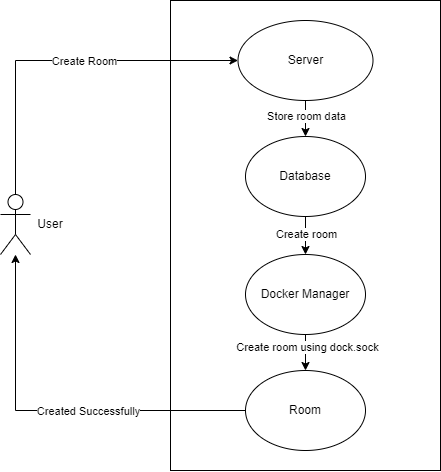
\includegraphics[scale=0.45]{usecase1.png}
						\centering
						\caption{Use Case Diagram for creation of a room}
						\label{fig:uc1}
					\end{figure}
				
					\paragraph{\normalfont{The Fig. \ref{fig:uc1} shows the use case of a user creating a room. The user requests the server to create a room. The server generates a unique identifier for the game sessions and notifies the docker manager to start the game session. The server stores the unique identifier and the docker manager stores the container information in the database. The created container acts as a server for the created game instance i.e., room. This room information is sent to the user upon successful creation. }}
					
					\begin{figure}[H]
						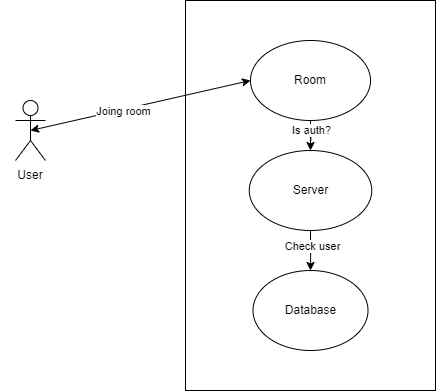
\includegraphics[scale=0.5]{usecase2.png}
						\centering
						\caption{Use Case Diagram for a user joining a room}
						\label{fig:uc2}
					\end{figure}
					
					\paragraph{\normalfont{The Fig. \ref{fig:uc2} shows the use case of a user joining a room. The user is authenticated and the identity is established. To connect to a private room, the user must provide the unique room identifier. Whereas, to connect to connect to a puiblic room, the user is connected to the closest room from a list open rooms. Once a user joins a room, the data is broadcasted to all the existing players in the room. }}
					
					\begin{figure}[H]
						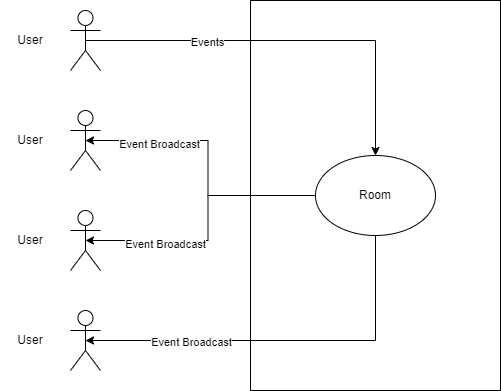
\includegraphics[scale=0.45]{usecase3.png}
						\centering
						\caption{Use Case Diagram for an action performed by a player}
						\label{fig:uc3}
					\end{figure}
					
					\paragraph{\normalfont{The Fig. \ref{fig:uc3} shows the use case of an action being performed by a player. The user actions are mapped to the events in the server and these events are broadcasted to other players to notify them about the changes brought about in the game by that action. This is a constant two-way communication between players and server to facilitate a seamless gameplay experience. }}
				
				\subsubsection{Sequence Diagram}
					\begin{figure}[H]
						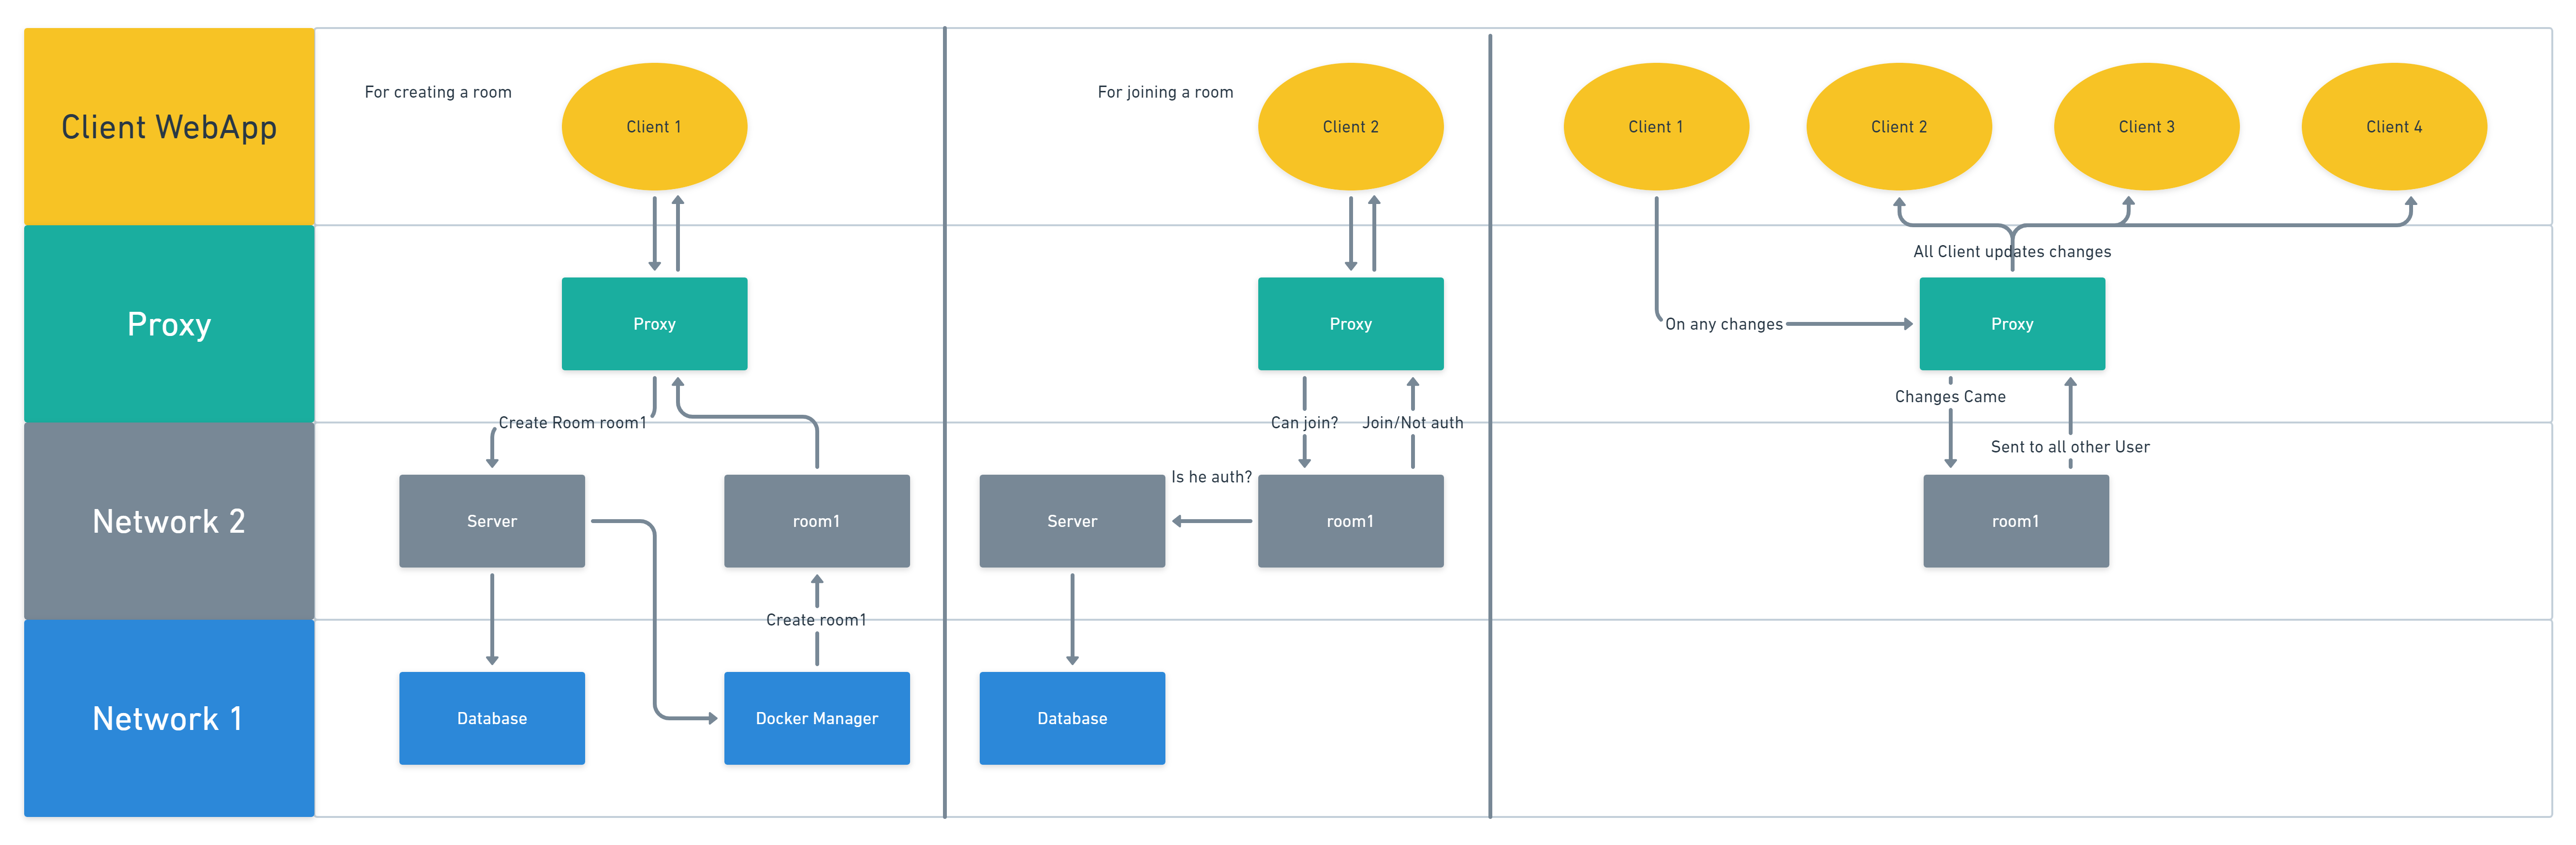
\includegraphics[width=15cm]{swimlane.png}
						\centering
						\caption{Sequence diagram for the project}
						\label{fig:seq}
					\end{figure}
				
					\paragraph{\normalfont{The sequence diagram for the project is as shown in Fig. \ref{fig:seq}. A sequence diagram chronologically shows the different events that occur throughout the life cycle of the game. }}
					
					\paragraph{\normalfont{The sequence diagrm shows the following events: }}
					\begin{enumerate}
						\item \textbf{Creation of a room: }A room is created upon the request of the user and the details are stored in the database. 
						\item \textbf{A user joining a room: }The user is authenticated and connected to the room. 
						\item \textbf{The game play: }The game states from one player is consistently broadcasted with the players in the room. 
					\end{enumerate}

	
	\chapter{Testing}
	\thispagestyle{fancy}
	
		\paragraph{\normalfont{This section provides an overview of testing, testing procedure, and test case information. Software testing is a mechanism for ensuring the proper functionality of software as well as determining whether or not the application fits the defined requirements. They verify that the application is bug and defect free. This ensures that the final consumer receives a high-quality product.}}
	
		\section{Test Workflow}
			\paragraph{\normalfont{Testing is done to uncover problems in the product at an early stage, before the product is put into production. Testing can be performed at various levels, such as module and sub-module. The entire product can be tested to guarantee proper module integration and that the product is fault-free from start to finish. There are numerous testing procedures available. These methodologies necessitate distinct strategies and test the numerous components that comprise the application.}}
			
			\paragraph{\normalfont{A variety of tests are run on the developed application before it is deployed. Tests are carried out to ensure that the application is carrying out the required duties correctly. A test suite is a collection of tests with a common goal. Fig. \ref{fig:test} shows the classification of testing methodologies. The methodologies that are relevant to our work are briefly described in the following sections. }}
			
			\begin{figure}[H]
				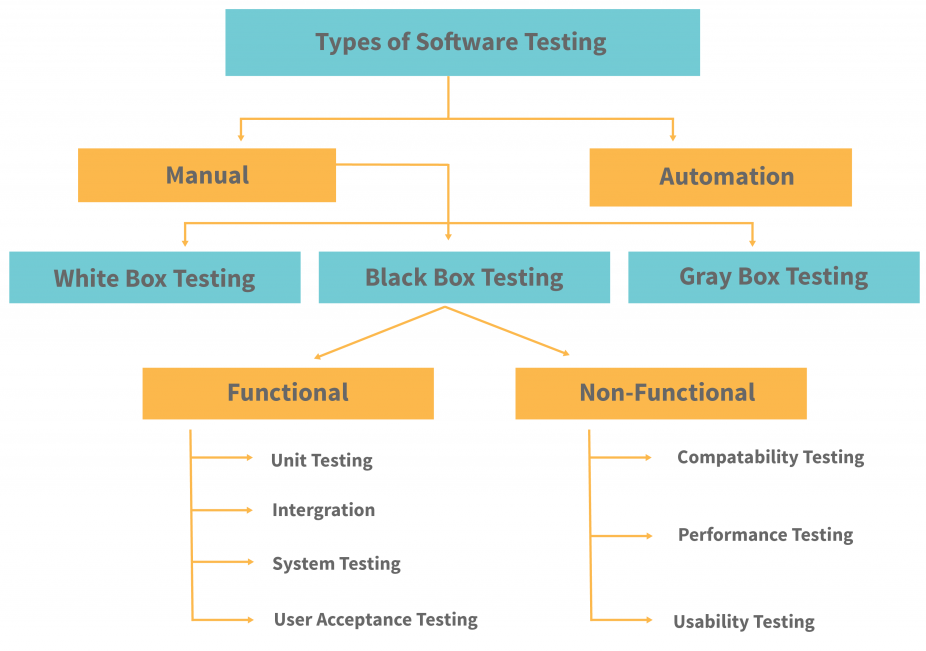
\includegraphics[width=15cm]{testing.png}
				\centering
				\caption{Classification of Testing Methodologies}
				\label{fig:test}
			\end{figure}
			
			
			\subsection{Objectives of Testing}
				\paragraph{\normalfont{The process of discovering defects in a program is known as testing. The purpose of the testing is to find errors that aren't immediately apparent to the developer or user but cause problems with the application's workflow. It is a way of detecting flaws or vulnerabilities in a code base in a methodical manner. The main advantage of testing is that it assures that the product fits the end-user criteria before it is issued for use. It also verifies that it is logically correct. Testing ensures that the application workflow is followed and that it functions as intended. The testing is done from the perspective of the users, thus all possible edge situations will be examined, lowering the danger of the application breaking.}}
				
			\subsection{Test Cases}
				\paragraph{\normalfont{The fundamental unit of the testing paradigm is the test case. They can be used to test a single entity, the functionality of a complete module, or the integration of the modules. To produce a more dependable product, additional test cases must be written to evaluate the application's end-to-end functionality while taking boundary conditions into account. A large number of test cases aids in determining the accuracy and efficacy of a project.}}
				
			\subsection{Black-Box Testing}
				\paragraph{\normalfont{Black box testing is another name for behavioural testing. This type of testing is largely concerned with the functionality of the application. In general, the individual performing black-box testing does not need to understand how the program works internally. This form of testing can handle the following types of errors.}}
				
				\begin{itemize}
					\item Errors caused by a missing or improper interface.
					\item Errors in choice of the data structure or the database used.
					\item Errors caused by data initialization and data exchange.
				\end{itemize}
			
			\subsection{White-Box Testing}
				\paragraph{\normalfont{White-box testing is a type of software testing that examines an application's internal structures or workings rather than its functionality. To design test cases in white-box testing, an internal perspective of the system as well as programming abilities are used. The tester selects inputs to exercise code routes and identify expected outputs. White-box testing can be used in the software testing process at the unit, integration, and system levels. Data flow within a unit, Data flow between units during integration, and Data flow between subsystems during a system-level test can all be tested. This testing methodology applies in the following situations: }}	
				
				\begin{itemize}
					\item Ensuring the proper functionalities of all the sub-modules. 
					\item Ensuring consistent behaviour the system even for boundary conditions. 
				\end{itemize}
			
			\subsection{Unit Testing}
				\paragraph{\normalfont{Unit testing is in charge of testing the application's most basic unit. A unit is a little piece of code that can be thought of as its own program. It is used to ensure the authenticity of a module by checking for faults. The basic operation of the modules and their sub-modules is validated. Module interactions are also checked to ensure that data is passed between modules as expected. Unit testing is carried out throughout the product development process. Following the completion of product development, the units are tested to ensure that they continue to function as intended.}}
				
			\subsection{Integration Testing}
				\paragraph{\normalfont{Integration testing is the stage of  testing in which related sub-modules joined and assessed as a group. Integration testing is used to determine whether a system or component meets the functional requirements. It happens after unit testing but before system testing. Integration testing takes as input unit-tested modules, collects them into bigger aggregates, applies tests described in an integration test plan to those aggregates, and outputs the integrated system suitable for system testing. Top-down or bottom-up integration testing might be used.}}
			
			\subsection{Functional Testing}
				\paragraph{\normalfont{Functional testing is a sort of black-box testing, where the test cases on a software component being tested is base on the specifications of the component. This testing method concentrates on the system's functional components while neglecting the logical features of the application.}}
		
		\section{Test Case Details}
			\subsection{Test Case ID: 1}
				\textbf{Unit to test: }Google OAuth login
				\newline
				\textbf{Test data: }User Credentials
				\newline
				\textbf{Expected Result: }The user is authenticated using Google OAuth. 
				\newline
				\textbf{Pass/Fail: }Pass
		
			\subsection{Test Case ID: 2}
				\textbf{Unit to test: }User Movement
				\newline
				\textbf{Test data: }Keyboard inputs from the user
				\newline
				\textbf{Expected Result: }The player character movements in the game reflects the user's keyboard input and this movement it is replicated across all the users in the room. 
				\newline
				\textbf{Pass/Fail: }Pass
				
			\subsection{Test Case ID: 3}
				\textbf{Unit to test: }User Attack
				\newline
				\textbf{Test data: }Spacebar input and mouse pointer position (for aiming) from the user
				\newline
				\textbf{Expected Result: }The player character fires a bullet when the spacebar is keyed in the direction of the mouse pointer and it is replicated across all the users in the room. 
				\newline
				\textbf{Pass/Fail: }Pass
				
			\subsection{Test Case ID: 4}
				\textbf{Unit to test: }Enemy Path-finding
				\newline
				\textbf{Test data: }Movement of the player character
				\newline
				\textbf{Expected Result: }The enemy characters moves towards the closest player character and it is replicated across all the users in the room. 
				\newline
				\textbf{Pass/Fail: }Pass
				
			\subsection{Test Case ID: 5}
				\textbf{Unit to test: }Generation of the game world: 
				\newline
				\textbf{Test data: }Null
				\newline
				\textbf{Expected Result: }A new game world (map) is procedurally created and is broadcasted to all the users.  
				\newline
				\textbf{Pass/Fail: }Pass
		
		\section{Results}
			\begin{figure}[ht!]
				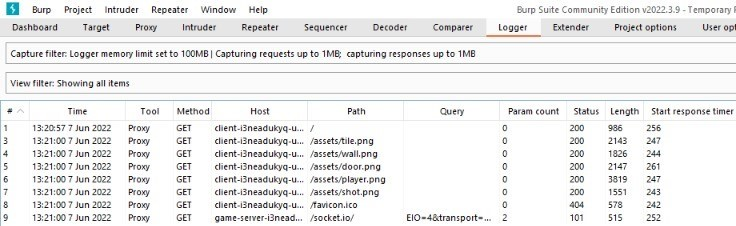
\includegraphics[width=15cm]{op1.jpeg}
				\centering
				\caption{Response time test result from BurpSuite}
				\label{fig:op1}
			\end{figure}
		
			\paragraph{\normalfont{Fig. \ref{fig:op1} shows the response time of client instances of the game as seen in BurpSuite. It can be seen that the response time is very low and is in the range of 240 - 250 milliseconds (ms). }}
		
			\begin{figure}[ht!]
				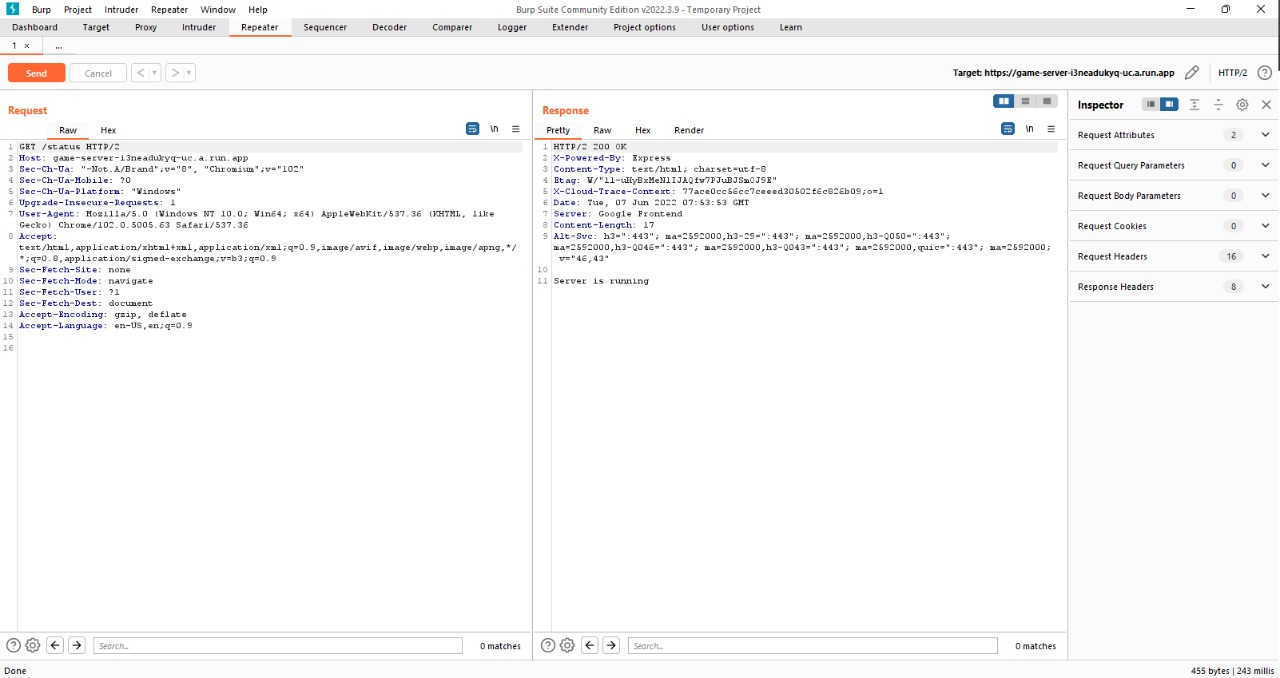
\includegraphics[width=16cm]{op3.jpeg}
				\centering
				\caption{Response time for WebSockets from BurpSuite}
				\label{fig:op3}
			\end{figure}
		
			\paragraph{\normalfont{Fig. \ref{fig:op3} shows the response time of the request from the server to the client as seen in BurpSuite. It can be seen that we have achieved a low response time of 243 (ms). }}
			
			
			
			\paragraph{\normalfont{Fig. shows the latency of the application as 236 (871 - 635) as seen from the Google Chrome inspect}}
			
			
		
			\paragraph{\normalfont{Fig. is a still from the game showing the movement of the player chracter in the room and some bullets being fired from it. }}
			
			
		
			\paragraph{\normalfont{Fig. shows the teleportation of the player characters. The still also shows the closure of the room boundary when all the player characters enter. }}
			
		
		
			\paragraph{\normalfont{Fig. shows some enemy characters swarming towards the player character. }}
			
	
	\chapter{Conclusions and Future Scope}
	\thispagestyle{fancy}
		
		\paragraph{\normalfont{The online multiplayer games constitute a significant portion on the gaming industry. With an active userbase of more than two billion players, the industry is worth around thirty thousand crores. Consequently, it is very important for the games to be highly scalable for meeting the evergrowing demands. To enhance user experience, it is crucial for the games to have low latency and feel more responsive.}}
		
		\paragraph{\normalfont{We have used docker containers for the game server. The containers allow us to easily manage, monitor and maintain the game server. They allow clound deployment, reduce latency by running an instance of the game on the cloud server nearest to the user, boost server performance by using multiple docker containers to run the server, it also enables support for rolling deployment and auto-scaling.}}
		
		\paragraph{\normalfont{We have built an online multiplayer game that allow users from across the globe to connect and play together. The game would be a 2D multiplayer game that supports features like orthogonal Top-down view, co-op combat, Character customization and public and private rooms for game sessions.}}
		
		\section{Future Scope}
		\paragraph{\normalfont{The following additional enhancements can be implemented in this project for better game-play experience: }}
		
			\begin{itemize}
				\item \textbf{Microtransactions: }A microtransaction is a business concept in which consumers can buy virtual goods for small sums of money. Microtransactions are frequently found in free-to-play games, which means there is no fee to download the game, only to purchase the online virtual products. Microtransactions are typically used to unlock certain features or to provide distinctive cosmetic, and occasionally game-changing, additions. 
				
				\item \textbf{Non-Fungible Tokens: } NFT-enabled games are blockchain games that allow users to buy in-game collectables to use as weapons to complete tasks or to sell to other users within the game and on external NFT marketplaces. Games with NFTs are not only exciting but also possibly rewarding. NFT gaming is growing fast, but more importantly NFT gamers are finding a purpose in their hobby. 
				
				\item Additional features like global leaderboards, weekly challenges, quests etc., can be added to the game.
			\end{itemize}
	
	\section*{}
	\pagebreak
	\addcontentsline{toc}{chapter}{Bibliography}
	\begin{thebibliography}{99}
		\thispagestyle{fancy}
		\bibitem{paper1} Cloud Gaming System in Docker Container Image:\newline \url{http://norma.ncirl.ie/4233/1/arunpugalendhi.pdf}
		
		\bibitem{paper2} Multi-platform Version of StarCraft: Brood War in a Docker Container: Technical Report: \newline \url{https://arxiv.org/pdf/1801.02193}
		
		\bibitem{paper3} Characterizing Docker Overhead in Mobile Edge Computing Scenarios: \newline \url{https://dl.acm.org/doi/pdf/10.1145/3094405.3094411}
		
		\bibitem{paper4} Enhancing Cloud Gaming User Experience through Docker Containers in Fog Nodes: \newline \url{http://norma.ncirl.ie/4135/1/manojkannan.pdf}
		
		\bibitem{paper5} The Future of Web and Mobile Game Development: \newline \url{https://bit.ly/3IPqDBI}
		
		\bibitem{paper6} The Development and Evaluation of Web-based Multiplayer Games with Imperfect Information using WebSocket: \newline \url{https://bit.ly/35C9ywK}
		
		\bibitem{link1} Phaser game engine documentation: \newline \url{https://newdocs.phaser.io/docs/3.55.2}
		
		\bibitem{link2} Phaser game engine tutorials: \newline  \url{https://phaser.io/learn}
		
		\bibitem{link3} Udemy course on game development using Phaser: \newline \url{https://bit.ly/3GJTW7d}
		
		\bibitem{link4} MMORPG academy course in Zenva: \newline \url{https://bit.ly/34P7ReU}
		
		\bibitem{link5} JavaScript and TypeScript tutorials: \newline \url{https://youtube.com/c/Ourcadehq}
	\end{thebibliography}
\end{document}